\chapter{Preparation}
\textit{In this chapter, I first state the software I used and the starting point for this project. I move on to present the formal requirements. This is followed by a discussion of the different components of a programmable data plane, including the P4 programming language, the SDNet compiler, the NetFPGA platform and the P4$\rightarrow$NetFPGA workflow. Finally, I discuss the project workflow.}

\section{Software Used}
Below I describe and justify, where necessary, the development environment and the programming languages that I used.

\subsection{Development Environment}
\begin{itemize}% [leftmargin=*] 0em: the starting letter is aligned, *: the dot is aligned.
	\item \textbf{The NetFPGA SUME}\footnote{A collaborative effort between Digilent, the University of Cambridge and Stanford University.} \cite{netfpgasume} is an open-source platform which provides an accessible development environment that both reuses existing codebases and enables new designs. It uses an advanced, FPGA-based board that features a Xilinx Virtex-7 690T supporting 30 13.1 GHz GTH transceivers. This board easily supports simultaneous wire-speed processing on the four 10Gb/s Ethernet ports, and it can manipulate and process data on-board, or stream it over the 8x Gen3 PCIe interface and the expansion interfaces. It is indeed ideal for any high-performance design such as in this project.
	
	\item \textbf{P4$\rightarrow$NetFPGA} (P4 on NetFPGA) is the workflow to develop and test P4 programs using the Xilinx\footnote{\url{https://www.xilinx.com/}} P4-SDNet\footnote{\url{https://www.xilinx.com/products/design-tools/software-zone/sdnet.html}} toolchain within the NetFPGA SUME reference switch design.
	
	\item \textbf{Vivado$^{\textrm{\textregistered}}$ Design Suite} is a software suite produced by Xilinx for synthesis and implementation of HDL designs. Vivado was used in the project because it is the design environment for FPGA products from Xilinx, and is tightly-coupled to the architecture of such chips. Its flexibility also enables me to simulate my design behaviour with different stimuli, synthesize the design to hardware and perform timing analysis.
	
	\item \textbf{Git} was used for version control, allowing quick roll-back and efficient management of multiple source trees using branches to implement different functionalities at various stages of the project. The repository itself was hosted remotely on GitHub\footnote{\url{https://github.com/ttbui11/part-ii-proj/}}.
	
	\item \textbf{Microsoft OneDrive}\footnote{\url{https://onedrive.live.com/about/en-gb/}} was used to back up relevant files throughout the project.
\end{itemize}

\subsection{Programming Languages}
In this project, I used a multitude of languages, including \textbf{P4}, \textbf{Verilog}, \textbf{Tcl} and \textbf{Python}.

\begin{itemize}
	\item \textbf{P4} \cite{bosshart2014p4} is a high-level language designed to describe packet processing logic in the packet forwarding planes. Besides, unlike general purpose languages such as C or Python, P4 is domain-specific with a number of constructs optimized around network data forwarding, hence is well-suited for implementing the forwarding plane of network elements such as our switch.
	
	\item \textbf{Verilog} was used to implement certain HDL modules within the NetFPGA platform, in order to add or modify certain functionalities to suit the purpose of my design. In fact, the NetFPGA platform is mostly Verilog-based, except for the packet-processing pipeline, which is implemented in P4. Thus, this project requires a strong grasp of Verilog. 
	
	\item \textbf{Tcl} was used as part of the Xilinx Vivado development environment to write project wrappers and debug scripts.
	
	\item \textbf{Python} is the language used in the existing test infrastructure since the other languages used are for the hardware level. It was used extensively in the evaluation because of the Scapy module \cite{scapy}, which enables the user to send, sniff, dissect and forge network packets. This capability allows me to write unit tests for my program by building customised packets, sending and checking them.
\end{itemize}

I also made use of the \texttt{make} build automation tool to automate project builds, tests and benchmarks.

\section{Starting Point} 
\label{sec:start}
This project uses the knowledge about TCP introduced in the Part IB \textit{Computer Networking} course and the experience in Electronic Computer-aided Design (ECAD) and working with a design-flow for Field Programmable Gate Arrays (FPGAs) from Part IB \textit{ECAD and Architecture Practical Classes}.

During the development of this project, I acquired further knowledge from the materials covered in the following courses:%
\begin{itemize}
	\item \textit{High Performance Networking} (Part III P51) --- Introduction to P4 and P4$\rightarrow$NetFPGA;%
	\item \textit{Principle of Communications} (Part II) --- TCP flow control and congestion control. Design choices for scheduling and queue management algorithms for packet forwarding;%
	\item \textit{\LaTeX \ and MATLAB} (Part II) --- Typesetting the project proposal and dissertation.%
\end{itemize}

In terms of familiarity, I had no prior experience with P4 and Tcl programming language, the NetFPGA platform and the P4$\rightarrow$NetFPGA workflow, and little experience in Verilog from the similar language SystemVerilog learnt in Part IB \textit{ECAD and Architecture Practical Classes}. Therefore, I had to spent some time learning the languages and the workflow. I had some prior experience in Python and Git from various projects and internships.

The NetFPGA platform provides an infrastructure for the project, and some reference codes. I used from this infrastructure the existing interfaces, DMA, and most of the HDL modules and externs, modifying some of them where appropriate, and wrote my own P4 code for the core functionalities of the design. This means that all the P4 code and the Python tests were written from scratch, while the code for the additional HDL modules and externs in Verilog, as well as the project wrappers in Tcl, are modified to suit the required functionalities from some of the current modules in the existing infrastructure.

\section{Requirements Analysis}
This project has one software deliverable---an implementation for a programmable switch that will retransmit a packet when it receives the third DUP ACK from the receiver---which includes codes for the following: data plane, control plane, simulation environment and test environment.

Below is a list of requirements and extensions for the deliverable, prioritised using \textit{MoSCoW} criteria \cite{moscow}:

\textbf{Must have}
\begin{itemize}
	\item Have an implementation of the switch's functionalities in P4. 
	\item The implementation works correctly in an SDNet simulation (block level simulation).
	\item The implementation works correctly in a SUME simulation (chip level simulation).
	\item The implementation works correctly in a hardware simulation.
	\item A performance evaluation of the design.
\end{itemize}

\textbf{Should have}
\begin{itemize}
	\item The switch will send a notification to the source if the retransmit fails.
	\item A performance evaluation in comparison to existing TCP fast retransmit mechanism.
\end{itemize}

\textbf{Could have}
\begin{itemize}
	\item The design will support more than a single flow, and support the configuration of flows to monitor.
	\item The design will support different packet sizes.
	\item The design has the ability to adaptively add or remove flows to monitor.
\end{itemize}

\textbf{Won't have}
\begin{itemize}
	\item The implementation will not be simulated using network simulators such as ns2 or omnet++.
\end{itemize}

\section{The P4 Language}
P4 (Programming Protocol-independent Packet Processors) has become the \textit{de facto} standard language for describing how network packets should be processed, and is becoming widely used by many developers in  conjunction with SDN control planes. This section gives a brief overview of the P4 programming language with the aim to provide sufficient basis to understand the project.

Most targets, if not all, implement both a control plane and a data plane. P4 is designed to specify only the data plane functionality of the target. P4 programs also partially define the interface by which the control plane and the data plane communicate, but P4 itself cannot be used to describe the control plane functionality of the target. Thus, in the remaining of this dissertation, when we refer to P4 as “programming a target”, we mean “programming the data plane of a target”. Figure \ref{p4target} describes the canonical process of programming a P4 target. The vendor of a packet processing device provides three components to the user:

\begin{itemize}
	\item The packet processing target device.
	\item A P4 architecture model to expose the programmable features of the target to the programmer.
	\item A compiler to map the user’s P4 program into a target-specific configuration binary file which is used to tell the target how it should be configured to process packets.
\end{itemize}

The programmer will write a P4 program to instantiate the architecture model, by filling its programmable components. The programmer also provides control software (i.e. a control plane) which is responsible for controlling the packet processing device at run time.

\begin{figure}[ht]
	\centering
	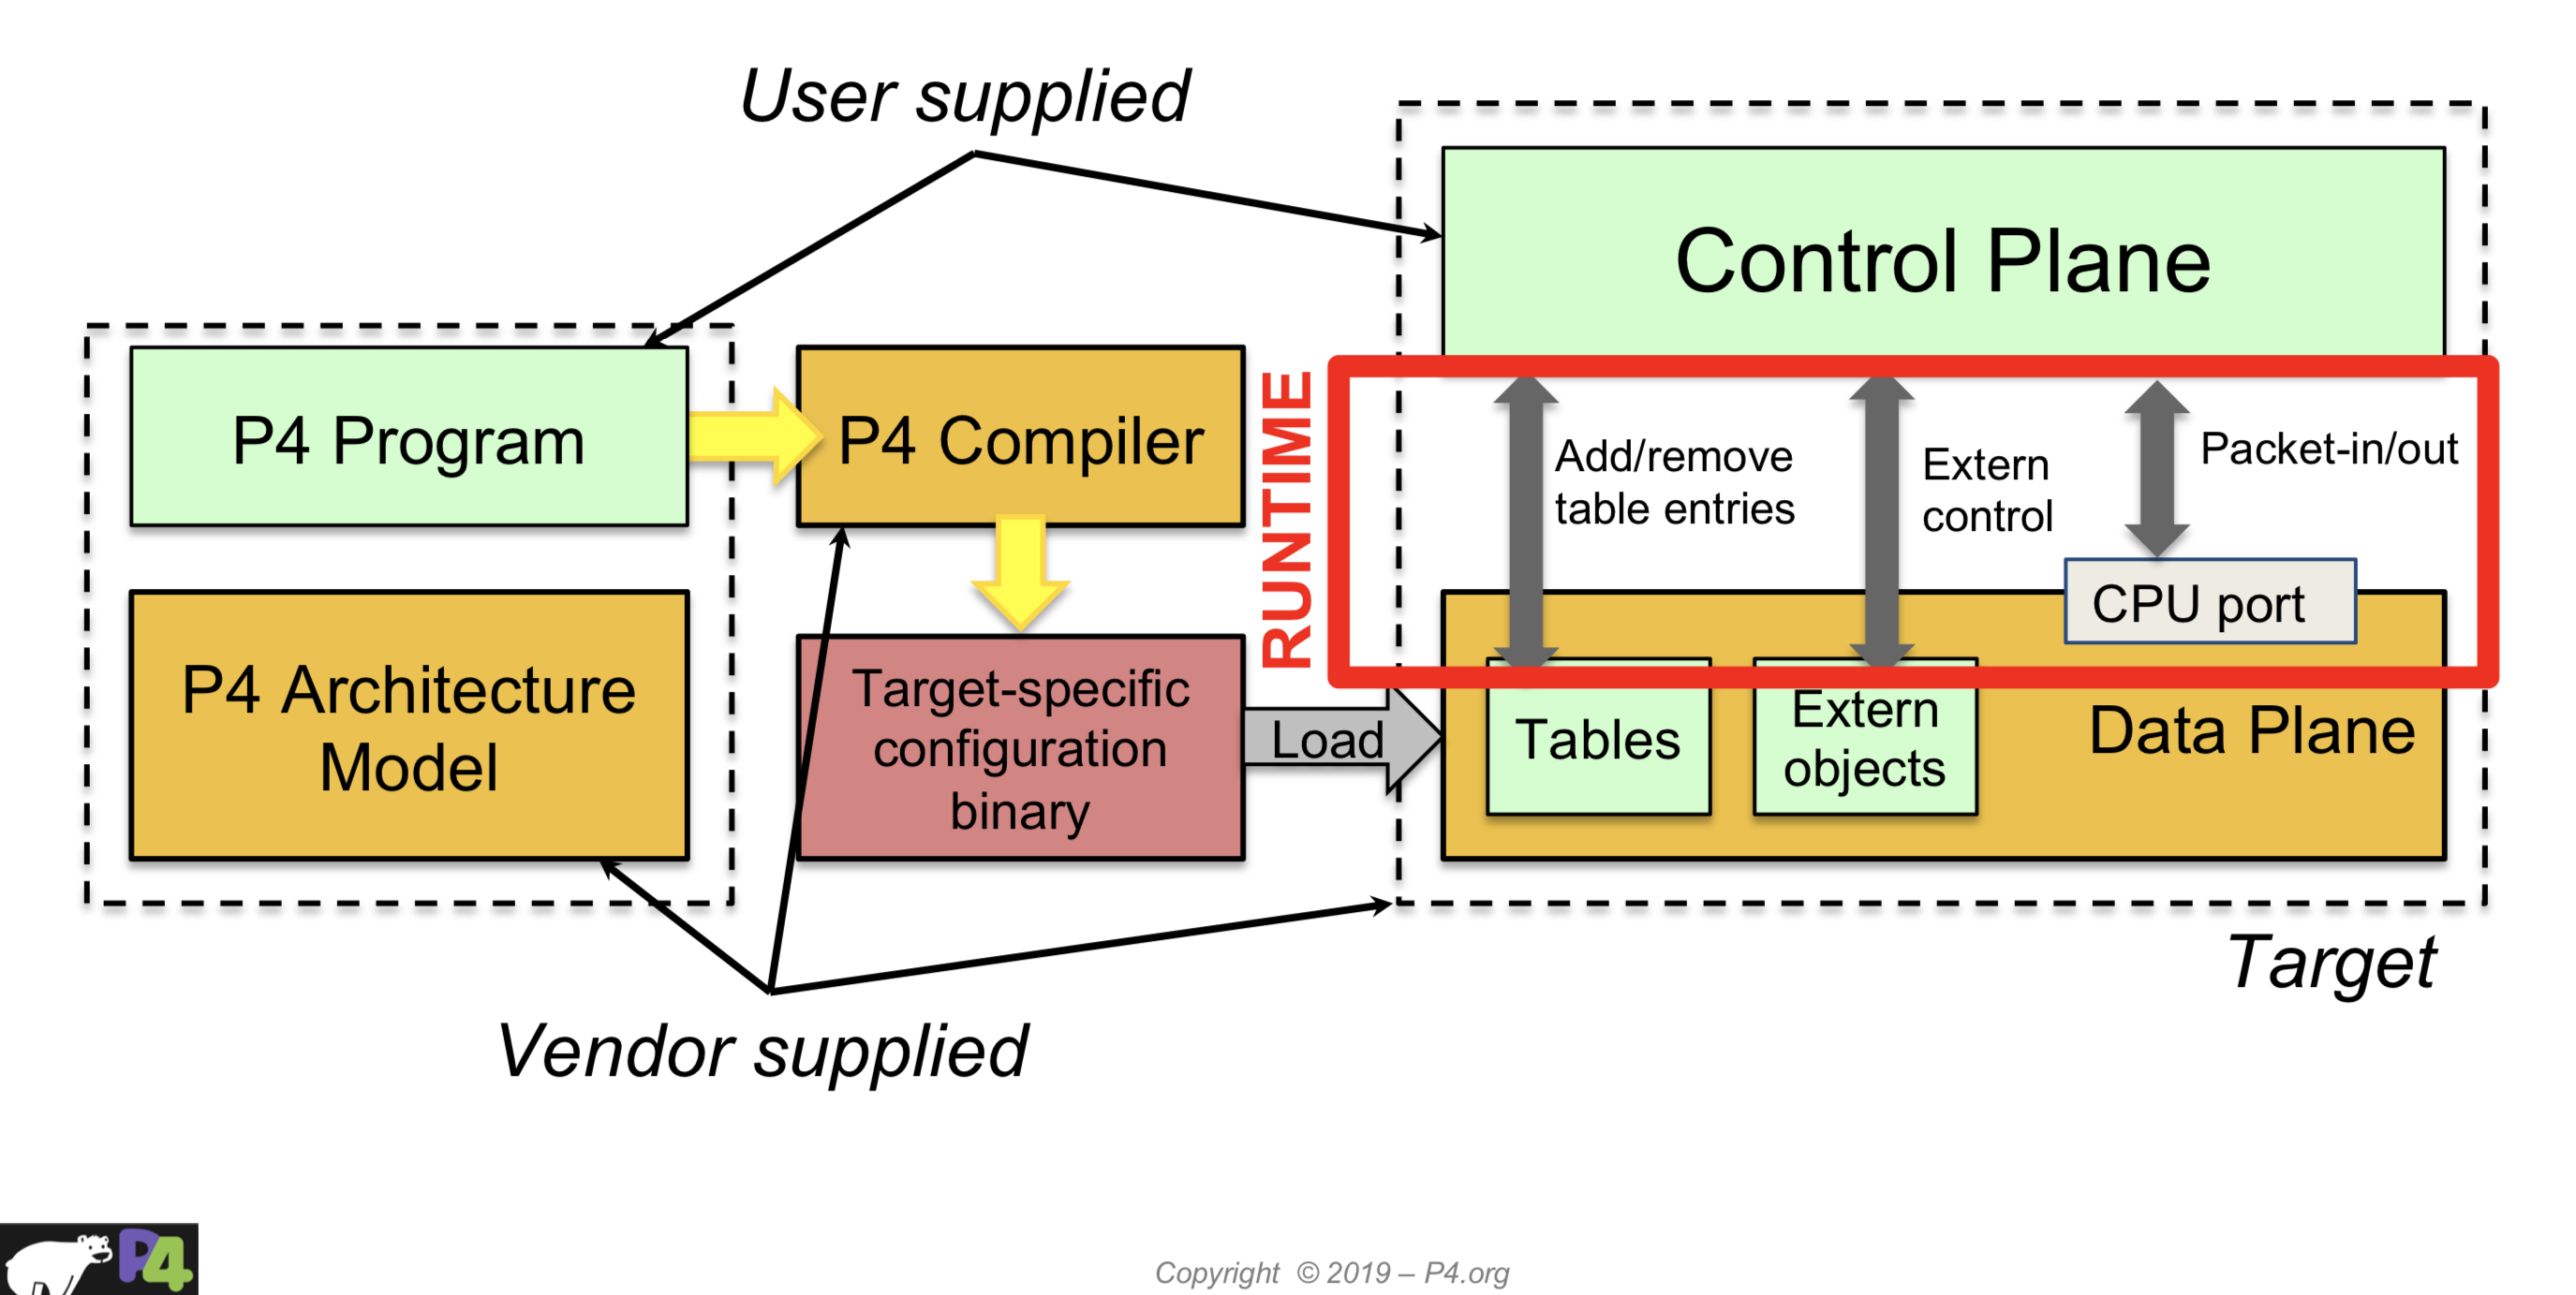
\includegraphics[width=\textwidth]{p4target.png}
	\caption{The process of programming a P4 target. Source: \href{https://p4.org}{P4.org -- Copyright \textcopyright\ 2019}.} 
	\label{p4target}
\end{figure}

In order to make the devices ``protocol-independent'', i.e. without built-in implementations of specific protocols, P4 allows us to define the format of all protocol headers that we want the device to handle using the \texttt{header} keyword. Here is an example that shows the definition of the Ethernet header in the project. The IPv4 and TCP headers are defined similarly. Note that \texttt{typedef} statements can also be used to make the code more readable.

{\renewcommand{\baselinestretch}{0.8}\small
	\begin{verbatim}
    typedef bit <48> EthAddr_t;
	
    header Ethernet_h {
      EthAddr_t dstAddr;
      EthAddr_t srcAddr;
      bit<16> etherType;
    }
	
    header IPv4_h {
      bit<4> version;
      ...
    }
	
    header TCP_h {
      bit<16> srcPort;
      ...
    }
	
    struct Parsed_packet {
      Ethernet_h ethernet;
      IPv4_h ip;
      TCP_h tcp;
    }
	\end{verbatim}
}

This makes P4-programmable switch differ from a traditional switch in two fundamental ways:
\begin{itemize}
	\item The data plane functionality is defined by the P4 programmer, rather than by the manufacturer of the switch. The data plane is configured at initialisation time to implement the functionality described by the P4 program and has no built-in knowledge of existing network protocols.
	\item The set of tables and other objects in the data plane are no longer fixed, but defined by the P4 program. The P4 compiler then generates the API that the control plane uses to communicate with the data plane, using the same channels as in a fixed-function device.
\end{itemize}

In this project, we will be using the SDNet compiler (``the compiler''), the NetFPGA SUME board (``the target device''), and the SimpleSumeSwitch architecture of the P4$\rightarrow$NetFPGA workflow (``the architecture model''), all of which will be described in more detail in the next three sections.

\section{The Xilinx SDNet}

\begin{figure}[!h]
	\centering
	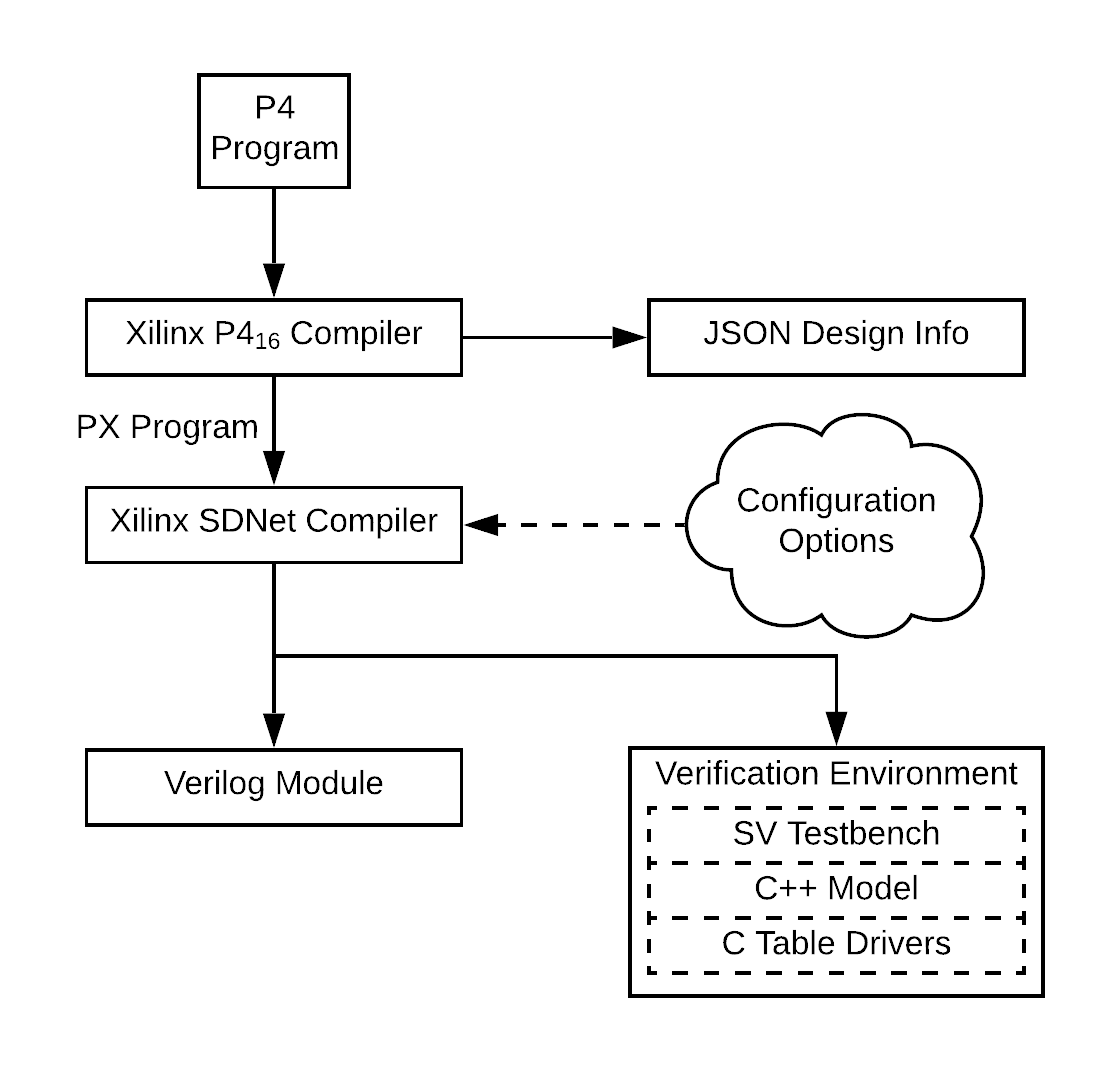
\includegraphics[width=0.7\textwidth]{sdnet.png}
	\caption{The Xilinx SDNet compilation flow. P4 programs are first translated into a PX program, which is then compiled into a Verilog module using the SDNet flow. SDNet also produces a verification environment.}
	\label{sdnet}
\end{figure}

The Xilinx SDNet compiler is the centerpiece of the P4$\rightarrow$NetFPGA workflow. It is the Xilinx SDNet original design environment for an internally-created packet processing language called PX \cite{px}, with a P4 to PX translator. Figure \ref{sdnet} depicts the process of compiling P4 programs that target the SimpleSumeSwitch architecture using SDNet. The front end translator maps P4 programs into corresponding PX programs and also produces a JSON file with information about the design that is required by the runtime control software. The PX program is passed, along with configuration parameters, into SDNet which then produces an HDL module that implements the user’s P4 program, and has standard AXI-Stream packet interfaces and an AXI-Lite control interface. SDNet generated designs can be configured to process packets at line rates between 1 and 400 Gb/s, hence is able to easily handle the aggregate 40G rate in the SUME reference switch design. SDNet also produces a SystemVerilog simulation testbench, C drivers to configure the PX tables, and an optional C++ model of the PX program to be used for debugging purposes.

\section{The NetFPGA Platform}
\begin{figure}[!h]
	\centering
	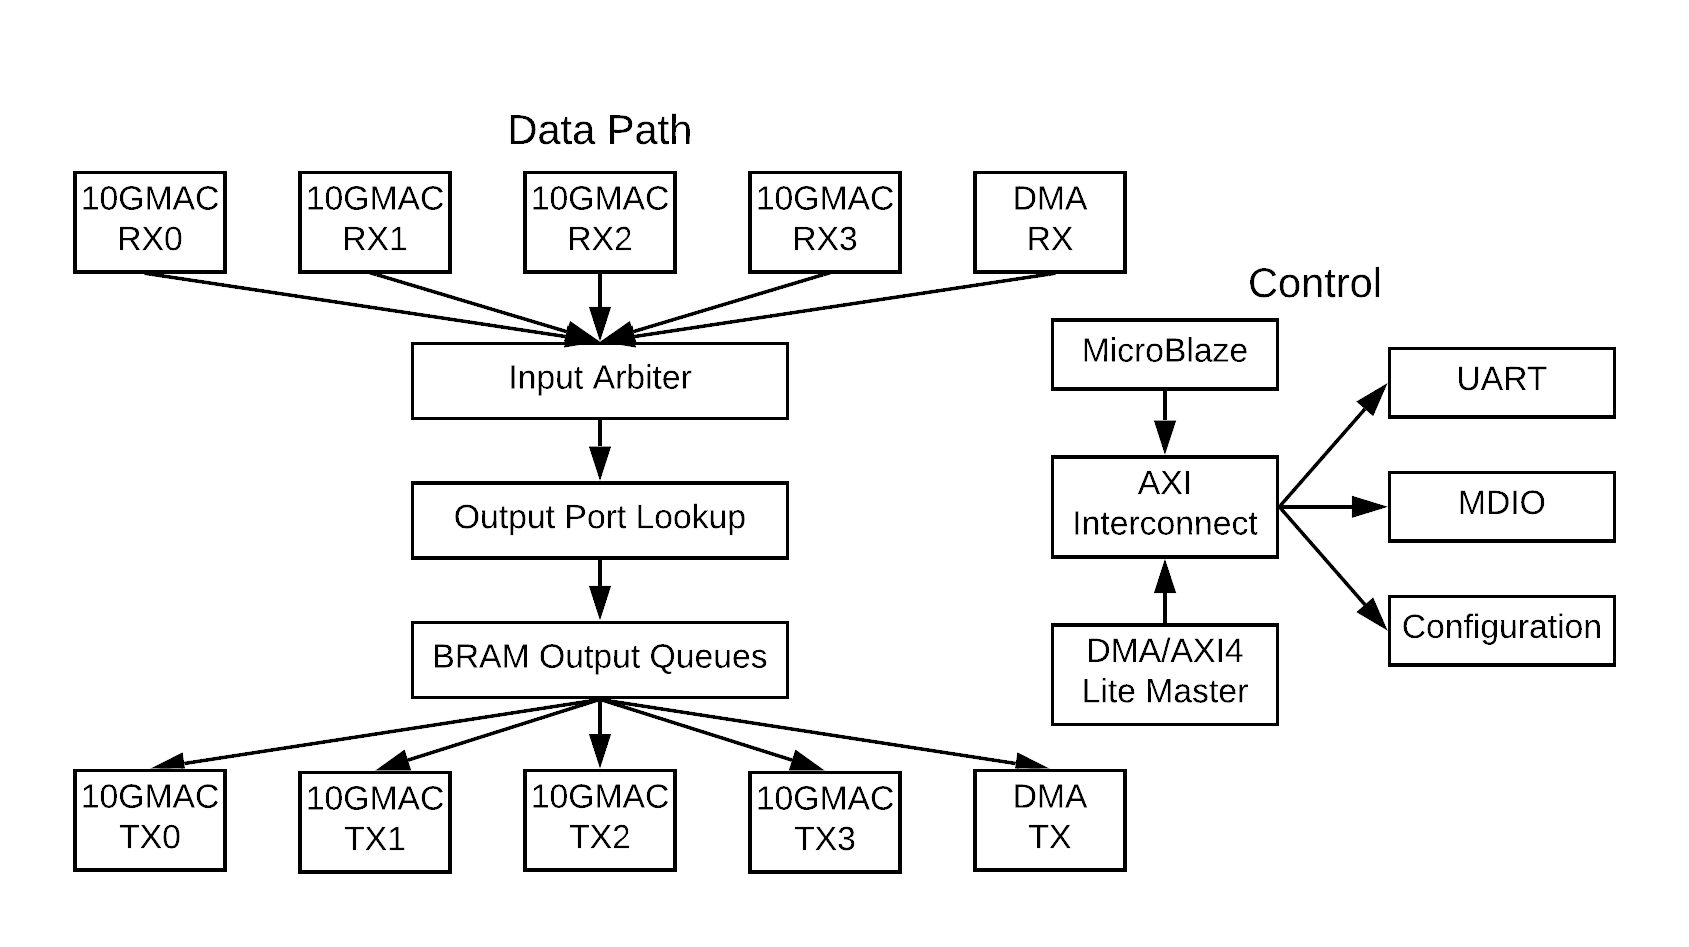
\includegraphics[width=\textwidth]{ref-switch.png}
	\caption{Block diagram of the NetFPGA reference design.}
	\label{ref-switch}
\end{figure}

The NetFPGA (Networked FPGA) project is a teaching and research tool designed to allow packets to be processed at line-rate in programmable hardware. It consists of four components: boards, tools and reference designs, a community of developers and contributed projects. The SUME board that was used in this project, which has I/O capabilities for 100 Gb/s operation such as NIC, multiport switch, firewall, or test/measurement environment, is the latest product in the NetFPGA hardware family. 

Figure \ref{ref-switch} depicts a block diagram of the canonical NetFPGA reference design which is used for switches, NICs, and IPv4 routers. It consists of four 10G SFP+ input/output ports along with one DMA interface for the CPU path. The NetFPGA data path consists of three main components: Input Arbiter, Output Port Lookup, and Output Queues. The Input Arbiter admits packets from the ports into the data path, towards the Output Port Lookup Module, where the main packet processing occurs and an output port is selected. The Output Queues buffer packets while they wait to be sent to the outputs. The core data path uses a 256-bit wide bus and runs sufficiently fast at 200 MHz to support an aggregate of 40 Gb/s from all four SFP+ ports.

The limitation of this platform is that it requires a substantial knowledge in both hardware design and networking, with programs written in Verilog or VHDL. To overcome this, the P4$\rightarrow$NetFPGA workflow was created to make it much easier to process packets in hardware and prototype new systems without being bogged down in hardware development.

\section{The P4$\rightarrow$NetFPGA Workflow}
\label{sec:p4-netfpga}
Figure \ref{fig:p4-netfpga} outlines the automated P4$\rightarrow$NetFPGA workflow \cite{fpga19}. We first write a P4 program which is compiled (by Xilinx P4-SDNet) into an HDL instance of the \textit{SimpleSumeSwitch} architecture. The SimpleSumeSwitch module is then automatically integrated into the NetFPGA reference switch design by replacing the default Output Port Lookup module.

\begin{figure}[ht]
	\centering
	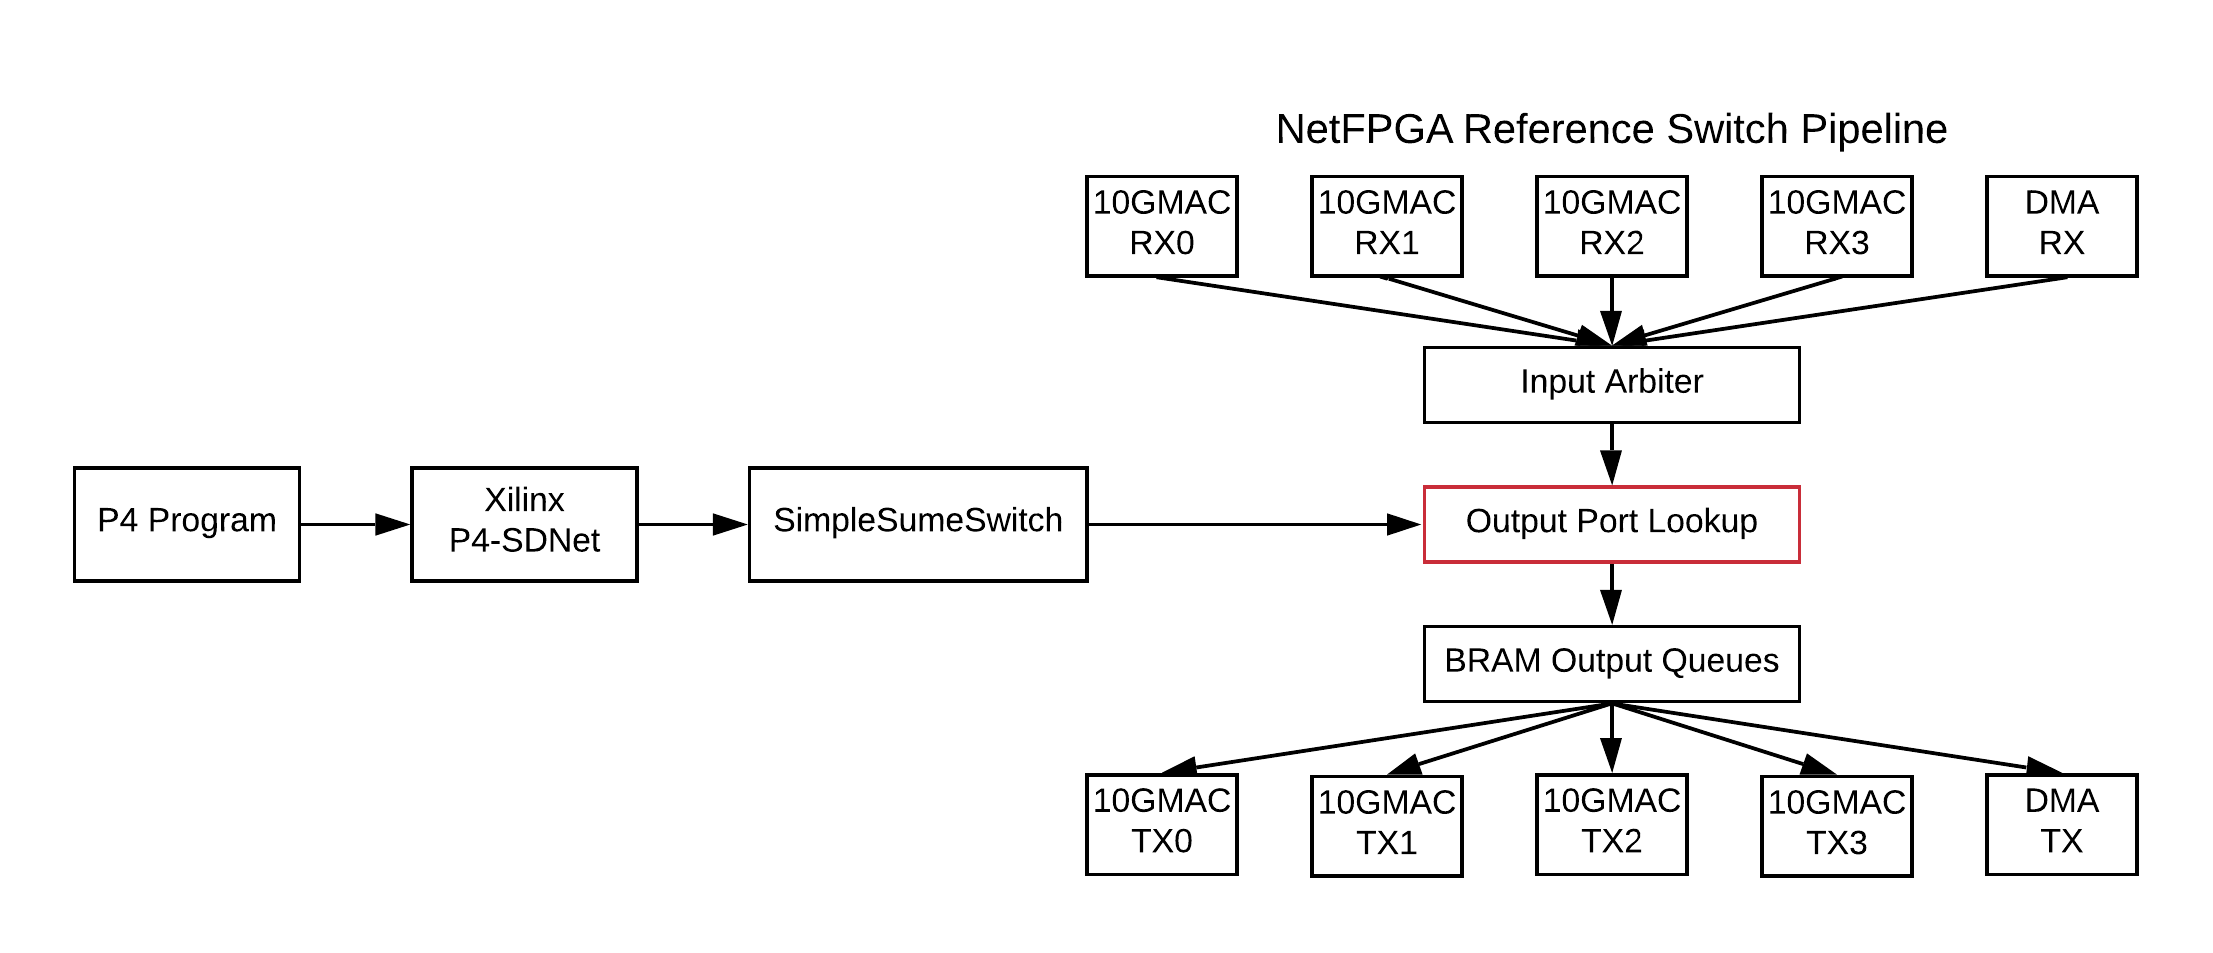
\includegraphics[width=\textwidth]{p4-netfpga.png}
	\caption{The automated P4$\rightarrow$NetFPGA compilation flow. P4 programs are compiled into an HDL instance of the SimpleSumeSwitch architecture, which is then used to replace the Output Port Lookup module in the NetFPGA Reference Switch Design.}
	\label{fig:p4-netfpga}
\end{figure}

The SimpleSumeSwitch is the P4 architecture that is currently defined for the NetFPGA SUME board. The architecture consists of a single parser, a single match-action pipeline, and a single deparser, as shown in Figure \ref{sss}.

The SimpleSumeSwitch’s \verb|sume_metadata| bus is defined as follows:

{\renewcommand{\baselinestretch}{0.8}\small
	\begin{verbatim}
    struct sume_metadata_t {
      bit<16> dma_q_size;     // measured in 32-byte words
      bit<16> nf3_q_size;     // measured in 32-byte words
      bit<16> nf2_q_size;     // measured in 32-byte words
      bit<16> nf1_q_size;     // measured in 32-byte words
      bit<16> nf0_q_size;     // measured in 32-byte words
      bit<8> send_dig_to_cpu; // send digest_data to CPU
      port_t dst_port;        // one-hot encoded (see below)
      port_t src_port;        // one-hot encoded (see below)
      bit<16> pkt_len;        // (bytes) unsigned int
    }
	\end{verbatim}
}

where the format of the \verb|dst_port| and \verb|src_port| fields is:

{\renewcommand{\baselinestretch}{0.8}\small
	\begin{verbatim}
    bit-7     bit-6     bit-5     bit-4     bit-3     bit-2     bit-1     bit-0
  (nf3_dma)-(nf3_phy)-(nf2_dma)-(nf2_phy)-(nf1_dma)-(nf1_phy)-(nf0_dma)-(nf0_phy)
	\end{verbatim}
}

and the functionality of each field is described by Table \ref{sume}. 

\begin{figure}[h]
	\centering
	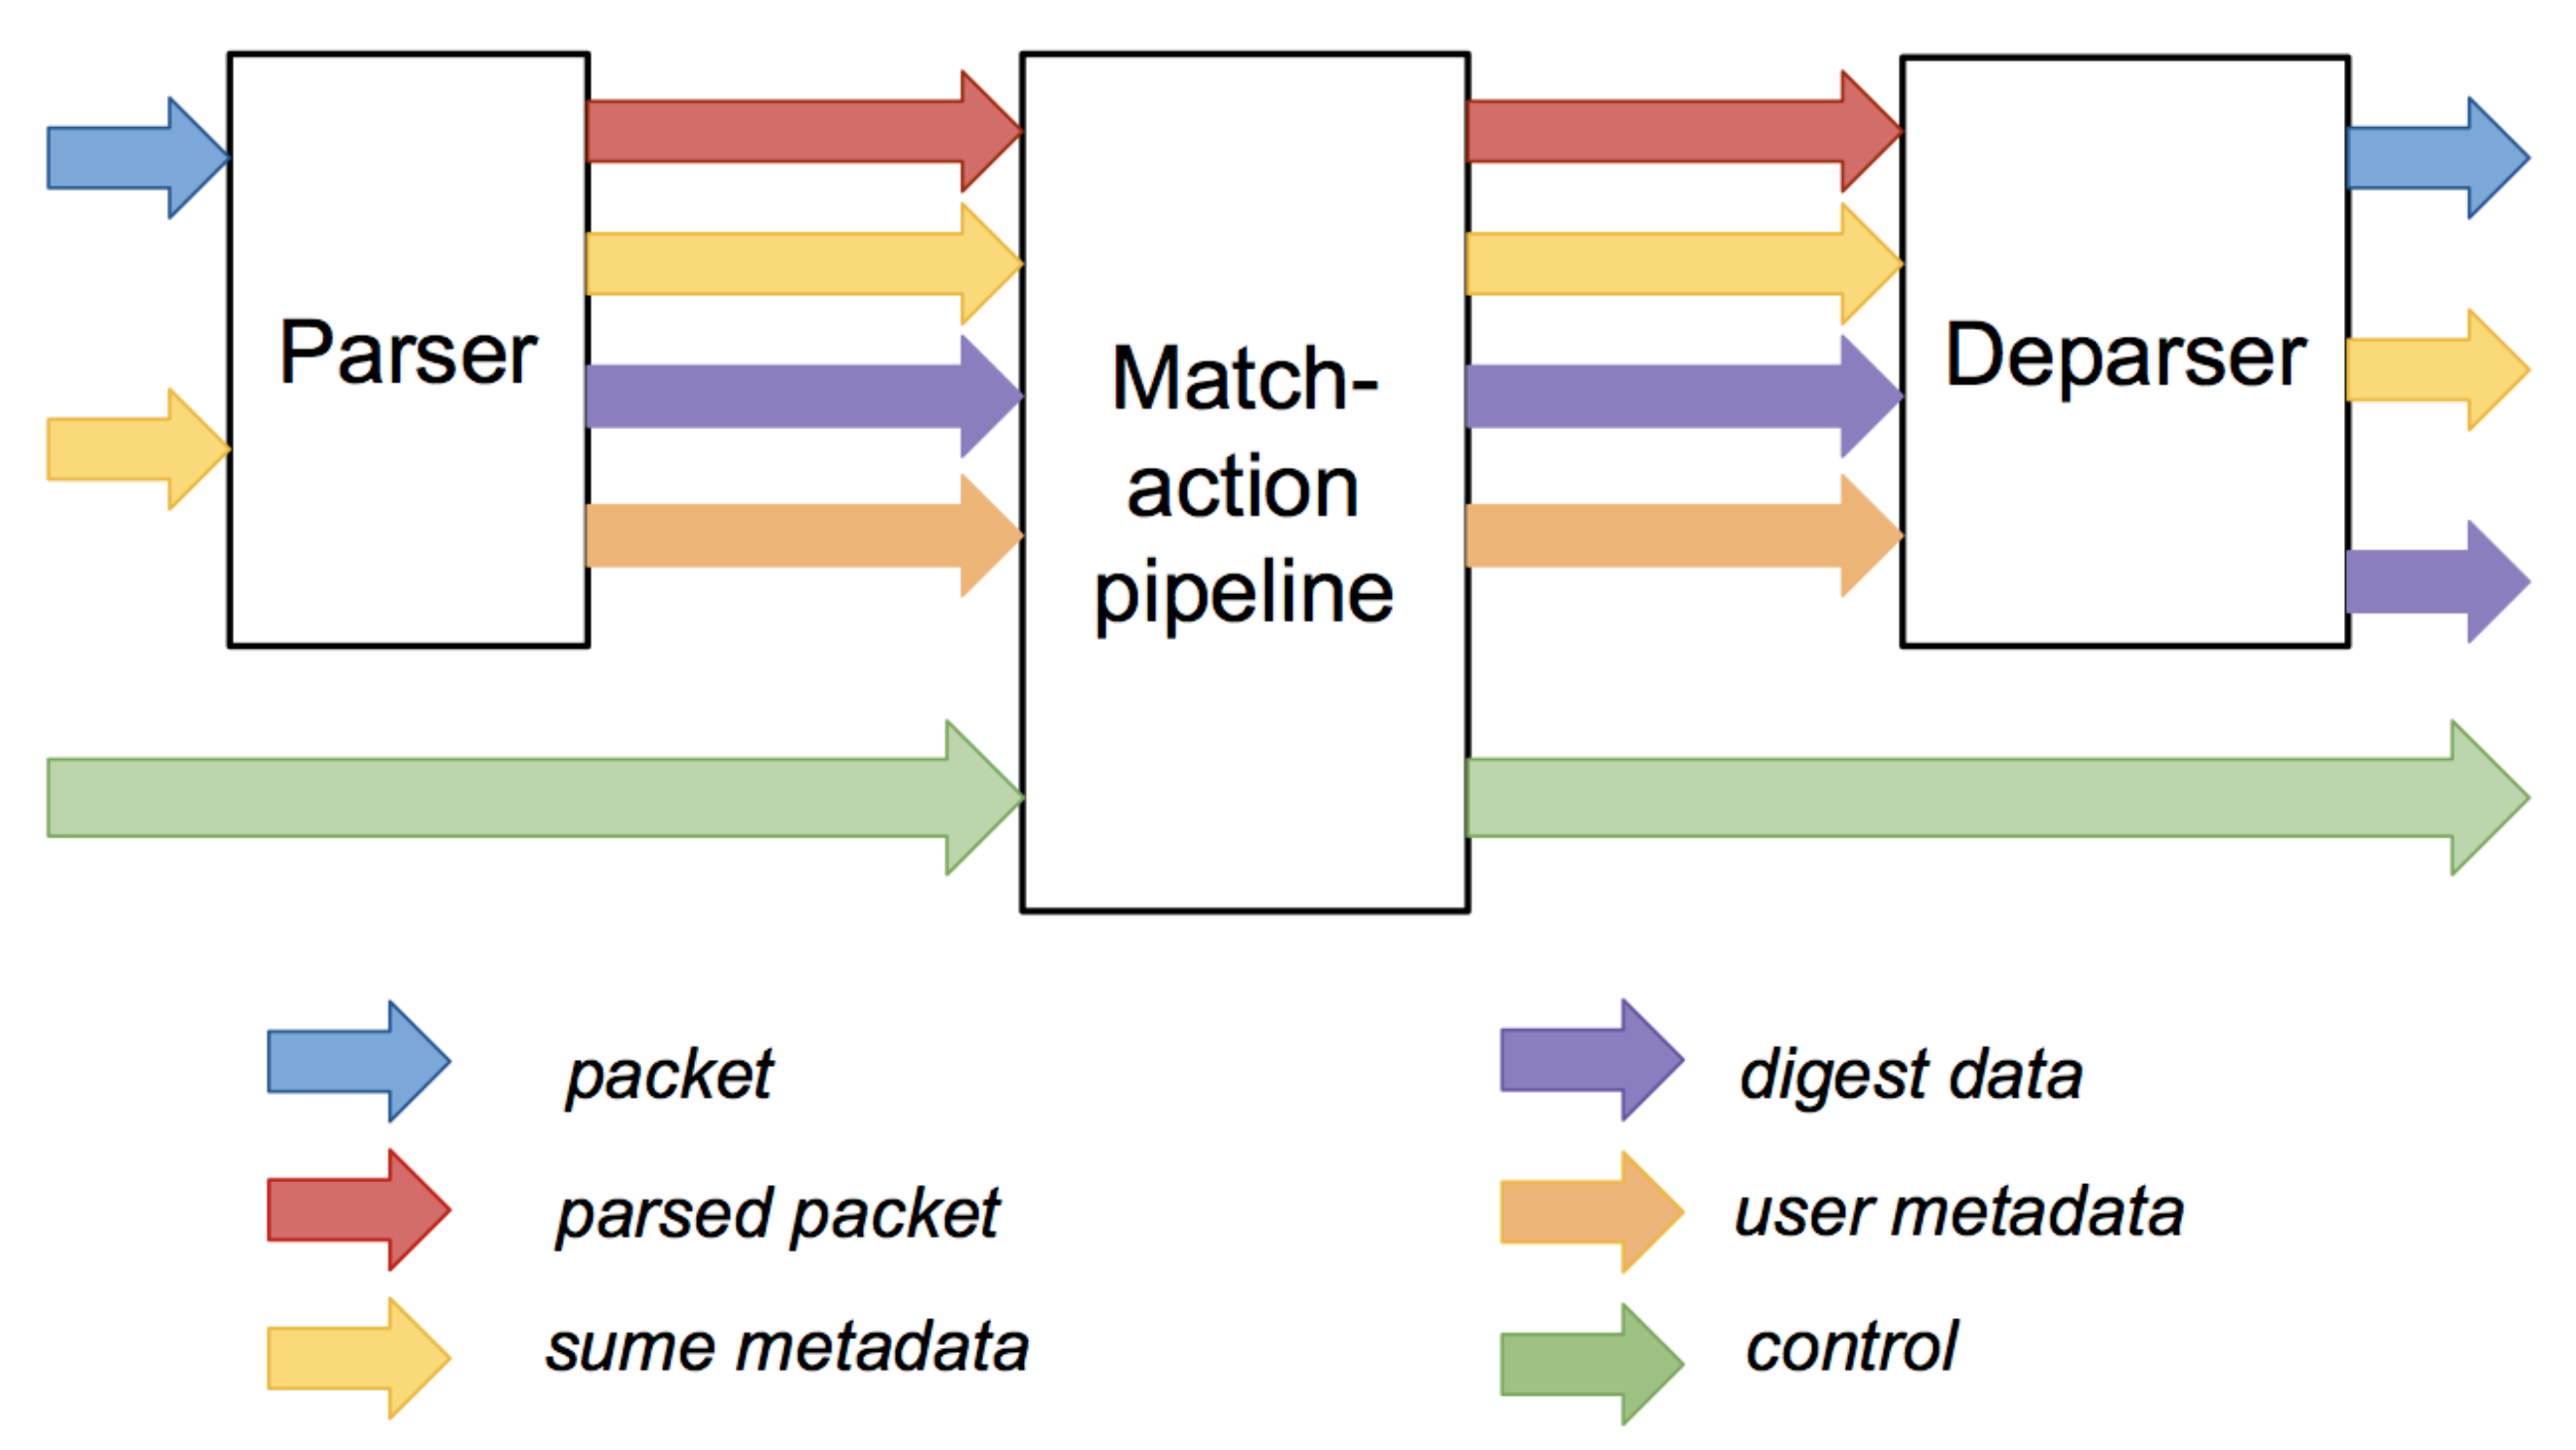
\includegraphics[width=0.9\textwidth]{sss.png}
	\caption{Block diagram of the SimpleSumeSwitch P4 architecture used within the P4$\rightarrow$NetFPGA workflow. Source: \href{https://github.com/NetFPGA/P4-NetFPGA-public/wiki/Workflow-Overview\#simplesumeswitch-architecture}{P4$\rightarrow$NetFPGA Home Wiki}.} 
	\label{sss}
\end{figure}

\begin{table}[ht]
	\begin{center}
		\caption{Description of the SimpleSumeSwitch \texttt{sume\_metadata} fields.}
		\label{sume}
		\begin{tabular}{ | c | c | p{10cm} |}
			\hline
			\textbf{Field Name} & \textbf{Size (bits)} & \multicolumn{1}{>{\centering\arraybackslash}m{10cm}|}{\textbf{Description}} \\ \hline
			\texttt{pkt\_len}  & 16 & Size of the packet in bytes (not including the Ethernet preamble or FCS) \\ \hline
			\texttt{src\_port} & 8 & Port on which the packet arrived (one-hot encoded) \\ \hline
			\texttt{dst\_port} & 8 & Set by the P4 program -- which port(s) the packet should be sent out of (one-hot encoded) \\ \hline
			\texttt{send\_dig\_to\_cpu} & 8 & Set the least significant bit of this field to send the \texttt{digest\_data} to the CPU \\ \hline
			\texttt{*\_q\_size} & 16 & Size of each output queue at P4 processing start time, measured in 32-byte words \\ \hline
		\end{tabular}
	\end{center}
\end{table}

The format of the \verb|digest_data| bus is defined by the P4 programmer. The \verb|digest_data| and the \verb|sume_metadata| together form to the \texttt{tuser} bus in the SUME reference switch design.

The format of the \verb|user_metadata| is also defined by the P4 programmer. It can be used to pass any additional information from the parser to the M/A pipeline and from the M/A pipeline to the deparser. The in/out \verb|control| signals are used to add/removed entries from tables and read/write control registers.

The SimpleSumeSwitch is a good architecture because it is simple and easy to understand, yet remains flexible enough to allow developers to implement a variety of different networking protocols and algorithms. Its flexibility also means that it could be extended or completely replaced by writing a new architectural model. For this project, I will modify the NetFPGA Reference Switch Pipeline to include a Cache Queue that will buffer packets. The customised architecture will be explained in more detail in  \S\ref{sec:arch-design}.

To sum up, the P4$\rightarrow$NetFPGA workflow includes the following steps:
\begin{enumerate}[label=(\arabic*)]
	\item Write P4 program.
	\item Implement custom extern modules, if any.
	\item Write Python scripts to generate test data for SDNet simulations.
	\item Run HDL simulations.
	\item Build bitstream for FPGA.
	\item Test the design on hardware.
\end{enumerate}

\section{Project Workflow}
\subsection{Preparation Stage}
The preparation stage happened in the first three weeks of the project. I spent the first week revisiting the basics of TCP and learning in depth its fast retransmit and recovery mechanisms. In the next two weeks, I learned the P4 language, set up the development environment and learned the P4$\rightarrow$NetFPGA workflow.

The P4 Language Consortium \cite{p4.org} provides a set of exercises to get me started. I completed their tutorial\footnote{\url{https://github.com/p4lang/tutorials}}, from which I learned the language basics such as basic forwarding and basic tunnelling. I also learned to use P4 tables and actions to implement advanced behaviour such as source routing and load balancing. 

Most of the time spent in setting up the NetFPGA environment went into getting approval for access to the live development repositories, including the P4$\rightarrow$NetFPGA and the NetFPGA-SUME codebase, and various licenses and tools necessary to use the P4$\rightarrow$NetFPGA toolchain (Xilinx P4-SDNet and Vivado Design Suite). Where appropriate, the licenses are quoted at the beginning of the file. The NetFPGA SUME board was already installed and configured, and is connected to a machine with the appropriate system requirements and dependencies located in the Computer Laboratory. To access the board from my personal device, I set up a Virtual Private Network (VPN) and \texttt{ssh} to the machine.

Finally, I learned the P4$\rightarrow$NetFPGA workflow through a series of exercises, provided by the NetFPGA Github Organisation\footnote{\url{https://github.com/NetFPGA}}. The workflow provides a template for a general P4 program following the SimpleSumeSwitch architecture model, from which I will start to write my implementation, as stated in \S\ref{sec:start}. The main challenge of this part is learning Verilog and Tcl in a short amount of time.

\subsection{Implementation Stage}
Following the preparation stage, the implementation stage of this project will take an iterative approach, as illustrated by the workflow in Figure \ref{fig:workflow}. After laying out the requirements and designing the architecture, I will start to write the implementation in P4 and test it by running an SDNet simulation, which is written in Python. Then, I will code the HDL modules and configure the system, which is followed by a SUME simulation. The next step will then be compiling the entire design into bitstream for FPGA programming and testing it in hardware, including a static timing analysis. All the steps are iterative: a code review is conducted after each ``Coding'' step and the outcome of each simulation step provides feedback for refining and improving the design in the next iteration. Finally, when the implementation passes all the tests, I will begin to evaluate its performance.

In order to fulfil the requirements analysis, I follow the \textit{spiral development model} \cite{spiral} with an iteration count equal to the number of major functionalities to add. This allows for continual implementation, testing and integration of the different functionalities.

\begin{figure}[!ht]
	\centering
	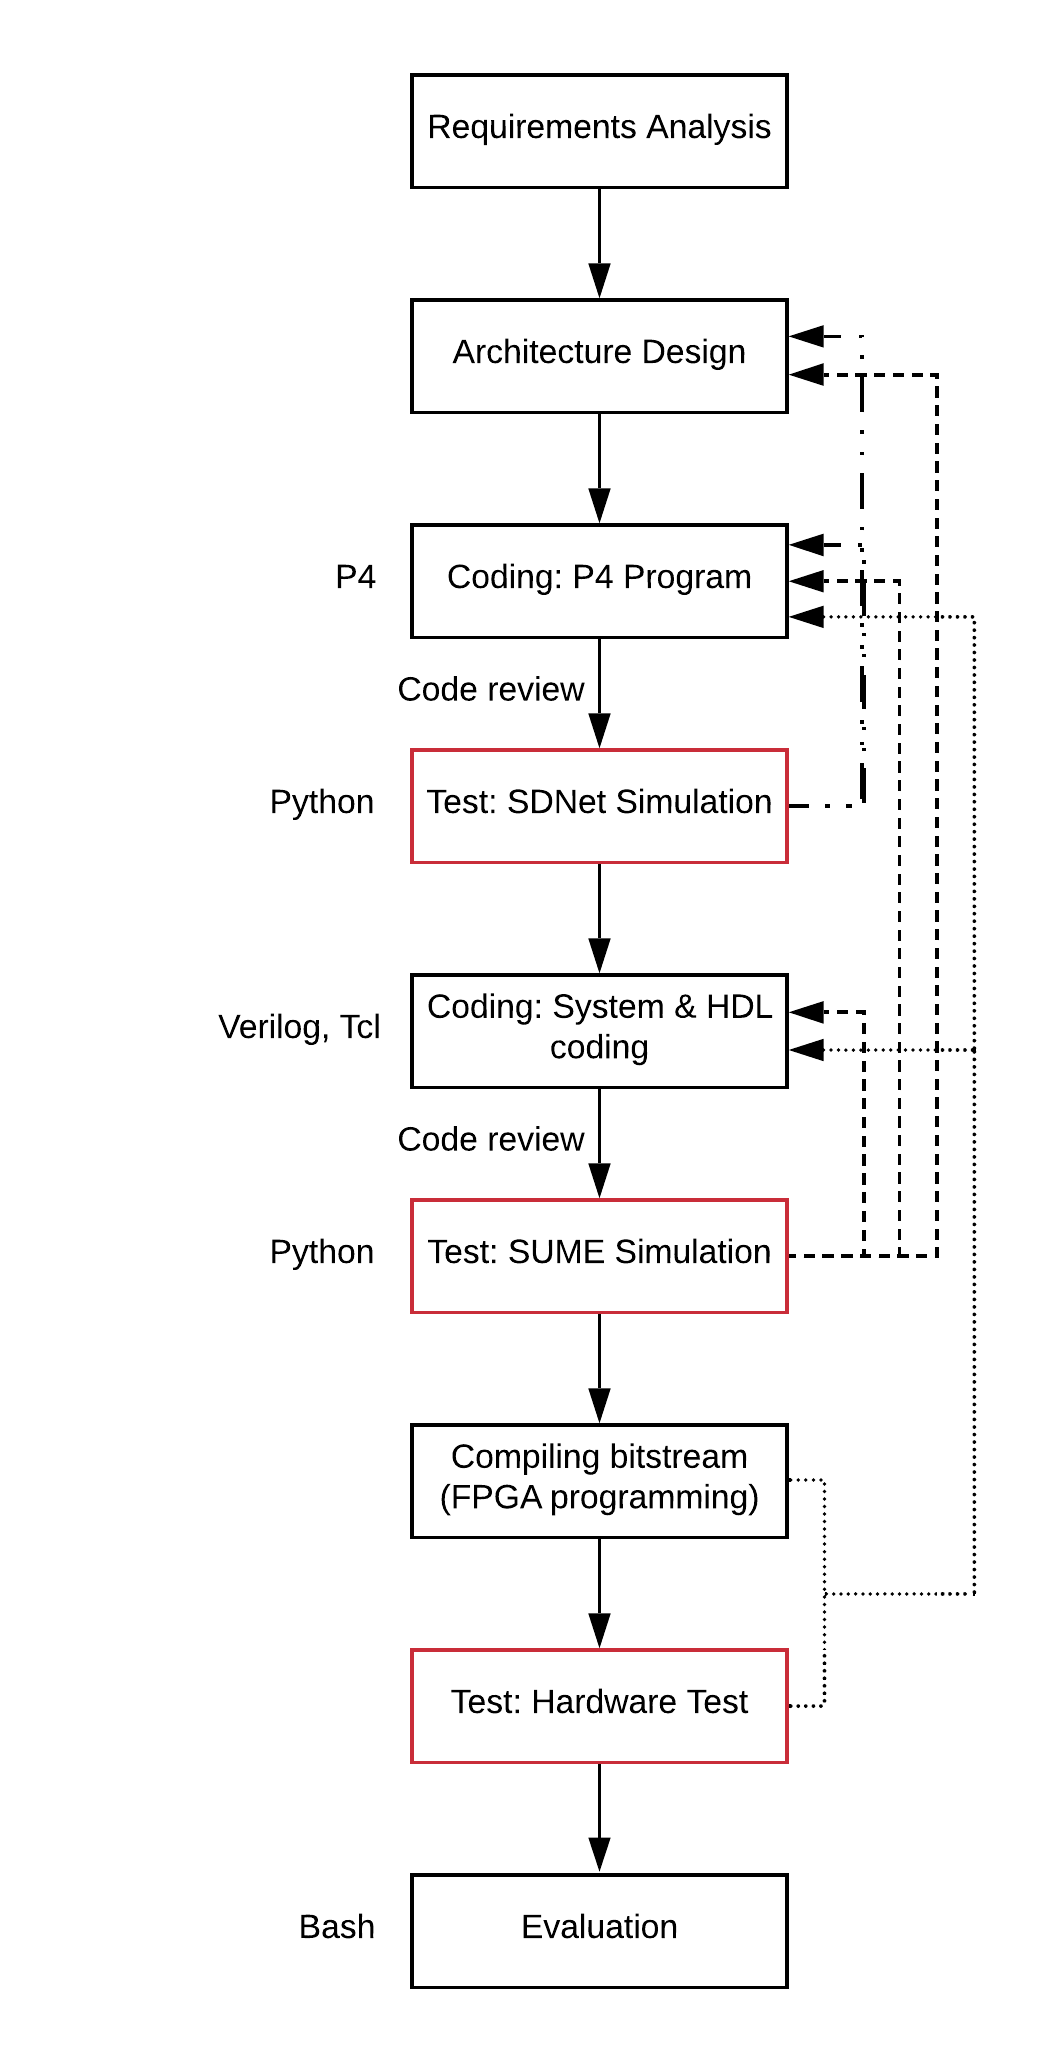
\includegraphics[width=0.75\textwidth]{workflow.png}
	\caption{Block diagram showing the workflow of the implementation stage. Dotted arrows represent a revision of previous steps, possibly with adjustments/refinements, in an iterative approach. Where appropriate, the programming language involved is stated. Passing all the steps in red box indicates the design meeting the requirements.}
	\label{fig:workflow}
\end{figure}

\subsection{Risk Analysis}
The P4$\rightarrow$NetFPGA workflow is a complex platform that required the knowledge of a multitude of languages, with limited documentation \cite{fpga} and community support \cite{support}. A potential risk for the project was the difficulty of being sufficiently proficient with the platform to modify its core components and hence the inability to implement the design. Complete failure to do so was unlikely, but it could have consumed a significant amount of development time. As suggested by the spiral development model \cite{spiral}, this high-risk part was scheduled early and some “catch-up” time was allocated in the project timetable in case it caused significant delays.

\subsection{Backup Plan}	
Throughout the project development, I made sure to follow good backup procedure by keeping local daily backups of my project using Time Machine for macOS. This provides recent history through incremental backups. I ensured additional remote storage by backing up with Microsoft OneDrive and Git, which also provided version control.